%%%%%%%%%%%%%%%%%%%%%%%%%%%%%%%%%%%%%%%%%%%%%%%%%%%%%%%%%%%%%%%%%%%%%%%%%%%%%%%%
%% BAKALÁRSKA PRÁCA                                                           %%
%%                                                                            %%
%% Názov (sk): Algoritmy detekcie a korekcie lokálnych                        %%
%%             znehodnotení digitálneho audio signálu                         %%
%% Názov (en): Algorithms for Detection and Correction of Local               %%
%%             Degradations in Digital Audio Signals                          %%
%%                                                                            %%
%% Autor: Jakub Kúdela                                                        %%
%% Vedúci: Mgr. Daniel Toropila                                               %%
%%                                                                            %%
%% Akademický rok: 2011/2012                                                  %%
%%%%%%%%%%%%%%%%%%%%%%%%%%%%%%%%%%%%%%%%%%%%%%%%%%%%%%%%%%%%%%%%%%%%%%%%%%%%%%%%

\chapter{Predstavenie algoritmov}
V rámci celej práce si najskôr zaveďme predpoklad, že lokálne znehodnotenie akéhokoľvek charakteru nepredlžuje ani neskracuje poškodenú časť pôvodného signálu. Algoritmy pripúštajúce skutočnosť, že lokálne znehodnotenia môžu zmeniť dĺžku trvania poškodeného úseku, sú oveľa komplexnejšie a nebudeme sa nimi ďalej zaoberať. Prv než si predstavíme obecný algoritmus pre reštaurovanie audio signálu poškodeného lokálnymi znehodnoteniami, si popíšme model reprezentácie digitálneho zvuku.

\section{Model reprezentácie digitálneho zvuku}
Algoritmy v práci počítajú s audio signálom ako s diskrétnou postupnosťou reálnych čísel predstavujúcich vzorky. Keďže algoritmy budú reštaurovať poškodené signály offline spôsobom, pod pojmom digitálny audio signál budeme chápať konečnú postupnosť vzoriek. V prípade, že $x$ je digitálny audio signál, jeho $n$-tú vzorku budeme značit $x_n$. Detailnejšie informácie ohľadom digitálnych audio signálov môžeme nájsť v úvodných kapitolách \cite{Godsill}.

\section{Modelovanie lokálnych znehodnotení}
V úvode sme si uviedli, že lokálne znehodnotenia môžu mať analógový aj digitálny charakter. Bolo vypozorované, že pôvodom analógové poškodenia majú odlišné správanie, než pôvodom digitálne. Tieto typy správania si zhrnieme do nasledovných dvoch modelov, z ktorých budeme v práci vychádzať:
\begin{itemize}
	\item \textit{aditívny} -- opisuje správanie lokálnych poškodení s analógovým pôvodom. Predpokladá, že vzorky lokálnych znehodnotení sú pričítané ku vzorkám pôvodného nepoškodeného signálu vo výsledný znehodnotený signál.
	\item \textit{nahradzujúci} -- opisuje správanie lokálnych poškodení s digitálnym pôvodom. Predpokladá že poškodené vzorky signálu sú úplne nahradené vzorkami lokálnych znehodnotení vo  výsledný znehodnotený signál.
\end{itemize}

\section{Obecný algoritmus}
Všetky reštaurátorské algoritmy zamerané na lokálne znehodnotenia, ktoré sa chystáme uviesť, majú niekoľko krokov spoločných. Zobecnenú schému týchto algortmov máme možnosť vidieť na obrázku~\ref{obrazok:obecny-algoritmus}.

\begin{figure}[!h]
	\centering
	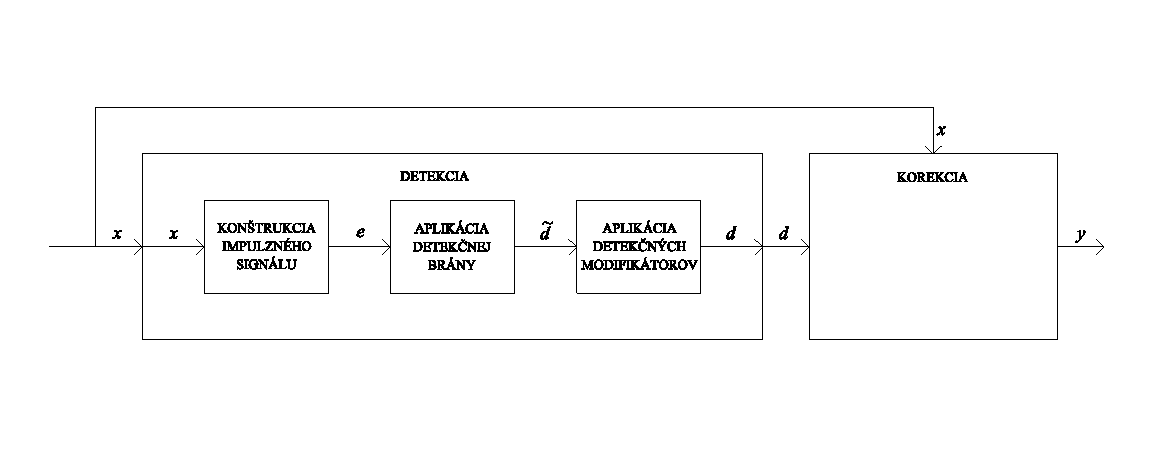
\includegraphics[width=1.0\textwidth]{images/obecny.eps}
	\caption{Schéma obecného algoritmu}
	\label{obrazok:obecny-algoritmus}
\end{figure}

Prácu vybraných algoritmov si môžeme rozdeliť na nasledovné fázy: 
\begin{itemize}
	\item \textit{detekcia} -- lokalizuje poškodené vzorky vstupného znehodnoteného signálu $x$ v podobe výstupného binárneho detekčného signálu $d$. Detekčný signál $d$ je definovaný nasledovým spôsobom:
	$$d_n = \left\{\begin{array}{l l}
		1 & \quad \text{$x_n$ je označená za poškodenú}\\
		0 & \quad \text{$x_n$ je označená za nepoškodenú.}\\
	\end{array} \right.$$
	
	Túto fázu si môže rozdeliť na ďalšie tri fázy:
	\begin{itemize}
		\item \textit{excitácia} -- zo vstupného poškodeného signálu $x$ skonštruuje odpovedajúci excitačný signál $e$. Excitačný signál $e$ má svojou intenzitou zobrazovať pravdepodobnosť poškodenia jednotlivých vzoriek poškodeného signálu $x$.
		\item \textit{aplikácia detekčnej brány} -- určí poškodenosť vzoriek znehodnoteného signálu $x$ z excitačného signálu $e$. Výsledkom aplikácie detekčnej brány na excitačný signál $e$ je prvotná detekcia v podobe binárneho celočíselného detekčného signálu $\tilde{d}$.
		\item \textit{aplikácia detekčného modifikátoru} (nepovinná fáza) -- upraví prvotnú detekciu $\tilde{d}$ na finálnu detekciu $d$. Cieľom aplikácie detekčného modifikátoru je kompenzácia nedostatkov prvotnej detekcie. Detekčných modifikátorov môže byť postupne na prvotnú detekciu $\tilde{d}$ aplikovaných aj viac.
	\end{itemize}
	\item \textit{korekcia} -- opravuje poškodené vzorky vstupného znehodnoteného signálu $x$ na základe detekčného signálu $d$. Výsledkom korekčnej fázy je výstupný opravený signál $y$.
\end{itemize}

Rozdielnosť vybraných algoritmov tkvie najmä v prístupoch ku excitácii a korekcii signálu. Detekčné brány a modifikátory môžu jednotlivé algoritmy zdielať, z toho dôvodu si ich uvedieme v práci až po predstavení vybraných metód. Pre jednotlivé algoritmy si zatiaľ uvedieme len popstupy pre excitáciu a korekciu signálu. Ku opisu detekčnych brán a modifikátorov sa dostaneme na konci tejto kapitoly. Prejdime teraz k predstaveniu algoritmov.

\section{Naivný algoritmus}
Prvý algoritmus, ktorý si uvedieme, je postavený na jednom z najtradičnejších analógových prístupov k čisteniu nahrávok poškodených lokálnymi znehodnoteniami. Vznikol pre účely reštaurovania nahrávok dochovaných na starších nosičoch. Jeho digitálnu variantu máme možnosť vidieť v niektorých súčasných hi-fi súpravách. Algoritmus stavia na predpoklade, že hľadané lokálne poškodenia majú prevažnú časť spektrálneho zastúpenia vo vyšších frekvenciách narozdiel od pôvodného signálu. Je to vďaka malému frekvenčnému rozsahu starších médií.

\subsection{Excitácia}
Naivný algoritmus získava excitačný signál $e$ zo vstupného poškodeného signálu $x$ vyseparovaním pásma vysokých frekvencií. Algoritmov podobného charakteru existuje mnoho, líšia sa typom použitého hornopriepustného filtru pre tieto účely. Naša metóda využije pri excitácii signálu jednoduchú a známu implementáciu hornopriepustného filtru\footnote{Preložené z anglického high pass filter.} založenú na diskrétnej aproximácií druhej derivácie. Tento filter môžeme nájsť v publikácii \cite{Kasparis} pojednávajúcej o algoritme, ktorý si predstavíme v poradí ako druhý. Motiváciou pre hľadanie druhej derivácie je, že derivácia produkuje vysoký výstup len v momentoch náhlych zmien signálu. Inými slovami povedané, zderivovaním signálu zmenšíme intenzitu v ňom obsiahnutých nižších frekvencií. Predpis pre diskrétnu aproximáciu druhej derivácie signálu a teda aj pre výpočet excitačného signálu je nasledujúci: 
$$e_n = x_{n-1} - 2 \cdot x_n + x_{n+1}.$$
Pre väčšiu dynamickú separáciu vyšších frekvencií vstupného poškodeného signálu je možné aplikovať vyššie uvedenú filtráciu opakovane.

\subsection{Korekcia}
Existuje mnoho naivných prístupov ku korekcii nahrávok obsahujúcich lokálne znehodnotenia. Niektoré metódy aplikujú na poškodené časti signálu dolnopriepustný filter\footnote{Preložené z anglického low pass filter.}, iné nahradia každú znehodnotenú vzorku signálu poslednou predchádzajúcou nepoškodenou\footnote{Metóda ``vzorkuj a podrž'', preložené z anglického ``sample and hold''.}. Náš naivný algoritmus sa ku korekcii bude stavať ako ku interpolačnému problému. Každú postupnosť poškodených vzoriek vstupného signálu nahradí vzorkami patriacimi pomyselnej úsečke, ktorá spája dve nepoškodené vzorky priamo susediace s postupnosťou. Formálne, naivným algoritmom opravený signál $y$ získame zo vstupného poškodeného signálu $x$ nasledovne:
$$y_n = \left\{\begin{array}{l l}
	x_n & \quad d_n=0\\
	(1-\frac{o_n}{g_n+1}) \cdot f_n + (\frac{o_n}{g_n+1}) \cdot r_n & \quad d_n=1\\
\end{array} \right.$$
kde $o$ a $g$ sú pomocné celočíselné signály definované nad detekčným signálom $d$:
$$o_n = \left\{\begin{array}{l l}
	0 & \quad d_n=0\\
	n - \max(\{\text{$i$ | $i\leq n$ a $d_i=0$} \}) & \quad d_n=1\\
\end{array} \right.$$
$$g_n = \left\{\begin{array}{l l}
	0 & \quad d_n=0\\
	\min(\{\text{$j$ | $j \geq n$ a $d_j=0$} \}) - \max(\{\text{$i$ | $i \leq n$ a $d_i=0$} \}) - 1 & \quad d_n=1\\
\end{array} \right.$$
a $f$ respektíve $r$ je signál získaný doprednou respektíve dozadnou korekciou spomenutou metódou nahradenia každej znehodnotenej vzorky signálu poslednou predchádzajúcou nepoškodenou:
$$f_n = x_{\max(\{\text{$p$ | $p \leq n$ a $d_p=0$} \})},$$ 
$$r_n = x_{\min(\{\text{$q$ | $q \geq n$ a $d_q=0$} \})}.$$
Táto interpolačná technika je v súčasnosti veľmi populárna vo voľne šíriteľnom software spolu s metódami, ktoré interpolujú sekvencie poškodených vzoriek pomocou Béziérových kriviek.

\section{Kasparis-Laneov algoritmus}
V roku 1993 bola zverejnená metóda, navrhnutá Takisom Kasparisom a Johnom Laneom \cite{Kasparis}, ktorá si podobne ako predchádzajúci algoritmus kládla za cieľ zbaviť staršie audio záznamy praskania. Tento algoritmus vznikol na báze predpokladu, že ku redukcii lokálnych znehodnotení zvukových nahrávok je možné pristupovať podobne ako ku redukcii šumu v digitálnych obrazoch\footnote{Šum ``soľ a korenie'', preložené z anglického salt and pepper noise.}. Veľmi obľúbená metóda na redukciu šumu v digitálnych obrazoch je aplikácia 2D mediánového filtru. Nahradzuje každý pixel digitálneho obrazu mediánom jeho okolitých pixelov. Aplikácia 2D mediánového filtru má však svoje nežiaduce vedľajšie účinky. Vyhladzuje aj oblasti nepoškodené šumom, čím degraduje kvalitu obrazu. Práve kvôli nežiaducej degradácií autori priamu filtráciu vylúčili a navrhli adaptívnu.

\subsection{Excitácia}
Prvý krok algoritmu, ku získaniu excitačného signálu $e$ zo vstupného poškodeného signálu $x$, je rovnaký ako jediný krok nášho naivného algoritmu. Na vstupný signál $x$ aplikujeme hornopriepustný filter založený na diskrétnej aproximácií druhej derivácie, čím získame signál $z$:
$$z_n = x_{n-1} - 2 \cdot x_n + x_{n+1}.$$
Autori metódy po pozorovaní výsledkov aplikácií filtru zistili, že vyfiltrovaný signál $z$ síce relatívne dôveryhodne vypovedá o umiestnení postupností znehodnotených vzoriek, ale nepremieta dostatočne dĺžku ich trvania. Ako ďalší krok preto navrhli aplikáciu operátoru lokálneho kvadratického priemeru na signál $z$:
$$w_n=\frac{1}{2 \cdot Q+1}\sum_{i=-Q}^Q z_{n+i}^2$$ 
kde $Q$ je celočíselný parameter určujúci veľkosť okolia vzoriek pre výpočet lokálneho kvadratického priemeru. Takto získaný signál $w$ pomenovali impulzný signálom. Pri zostavovaní algoritmu sa aplikácia operátoru lokálneho kvadratického priemeru ukázala ako vhodnejší krok, než aplikácia operátoru lokálneho priemeru absolútnej hodnoty vzoriek. Pre získanie excitačého signálu $e$ potrebujeme impulzný signál $w$ na záver znormalizovať jeho referenčným základom $b$. Referenčný základ impulzného signálu $w$ získame aplikáciou rekurzívneho filtru:
$$b_n=med(b_{n-R}, b_{n-(R-1)}, \cdots, b_{n-1}, w_n, w_{n+1}, \cdots, w_{n+R})$$ 
kde $R$ určuje rozsah okolia vzoriek pre výpočet lokálneho mediánu. Keďže je v danej situácií potrebný výpočetne náročný filter, počítajúci v relatívne veľkom okolí, doporučili autori pre efektívnejší výpočt $b$ najskôr zredukovať vzorkovaciu frekvenciu impulzného singálu $w$ celočíselným koeficientom $K$. Redukciou vzorkovacej frekvencie sa efektívne výpočetné okolie rekurzívneho mediánového filtru rozšíri $K$-násobne a tým pádom môže byť výpočet $b$ realizovaný s relatívne menšími parametrami $R$. Excitačný signál $e$ získame nakoniec zo vzťahu: 
$$e_n = \frac{|w_n - b_n|}{b_n}.$$ 
Výsledný signál $e$ je oproti impulznému profilu $w$ údajne prispôsobivejší voči hlasitostným a frekvenčným zmenám v nahrávkach. Schému opísaného procesu môžeme vidieť na obrázku~\ref{obrazok:kasparis-lane}.

\begin{figure}[!h]
	\centering
	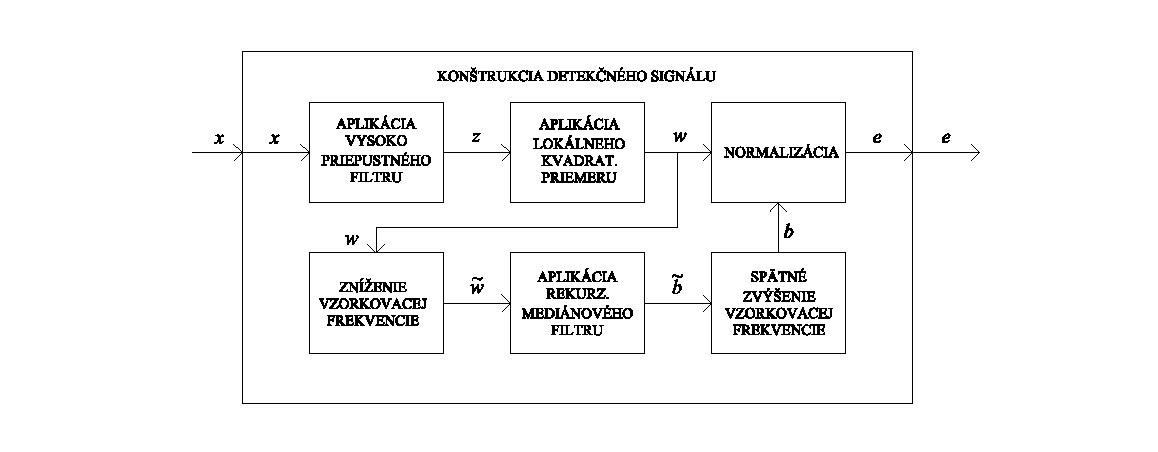
\includegraphics[width=0.8\textwidth]{images/kasparis.eps}
	\caption{Kasparis-Lane: schéma excitácie}
	\label{obrazok:kasparis-lane}
\end{figure}

Pre redukciu vzorkovacej frekvencie signálu $w$ autori algoritmu doporučujú metódu decimácie, ktorú však ďalej nerozvádzajú. V krátkosti si popíšme jednoduchú decimačnú metódu. Potrebné zmenšenie vzorkovacej frekvencie\footnote{Preložené z anglického downsampling.} celočíselným koeficientom $K$ dosiahneme preriedením $l$-vzorkového signálu impulzného profilu $w$ na $\tilde{l}$-vzorkový signál $\tilde{w}$, kde $\tilde{l}=\lceil \frac{l}{K} \rceil$, predpisom: $\tilde{w}_n=w_{n \cdot K}$. Spätné zväčšenie vzorkovacej frekvencie\footnote{Preložené z anglického upsampling.} $\tilde{l}$-vzorkového signálu referenčného základu $\tilde{b}$ (získaného z $\tilde{l}$-vzorkového impuzlného profilu $\tilde{w}$) celočíselným koeficientom $K$ na $m$-vzorkový signál referenčného základu $b$, kde $m=\tilde{l} \cdot K= \lceil \frac{l}{K} \rceil K$, docielime repetizáciou vzoriek: $b_n=\tilde{w}_{\lfloor \frac{n}{K} \rfloor}$.

\subsection{Korekcia}
Pri korekcii autori vylúčili mediánový filter úplne. Myšlienkou bolo aplikovať filter len na znehodnotené vzorky vstupného signálu. Po prevedení sérií experimentov usúdili, že najkvalitnejšie korekčné výsledky sú dosiahnuté aplikáciou mediánového filtru vtedy, keď filter počíta v malých okoliach zahŕňajúcich celé postupnosti poškodených vzoriek. Ako rozumný argument podali fakt, že keď je výpočetné okolie väčšie než postupnosť poškodených vzoriek, sú nové vzorky počítané z väčšej časti signálu a nemodelujú dobre lokálne hodnoty pôvodného signálu. Definitívne riešenie Kasparisa a Lanea pre korekciu poškodených vzoriek je aplikácia adaptívneho mediánového filtru s predpisom: 
$$y_n= med(x_{n-g_n}, \cdots, x_{n+g_n})$$ 
kde $g$ je pomocný celočíselný signál získaný z detekčného signálu $d$ spôsobom popísaným pri naivnom algoritme.


\section{Autoregresívny algoritmus}
V priebehu hľadania efektívnych algoritmov pre detekciu a korekciu lokálnych poškodení digitálnych audio nahrávok sa riešenia začali predovšetkým sústreďovať okolo štatistických prístupov. Štatistické metódy začali nadobúdať experimentálne najlepšie výsledky. Spomedzi pristúpov k signálu ako k časovej rade, je najpopulárnejším autoregresívne modelovanie\footnote{Preložené z anglického autoregressive (AR) modeling.}. Nasledované je kombinovaným autoregresívnym modelovaním s kĺzavými priemermi\footnote{Preložené z anglického autoregressive–moving-average (ARMA) modeling.}. Čisté autoregresívne modely modelujú náhodné procesy, ktorých hodnota v danom čase je váženou sumou konečného počtu bezprostredne predchádzajúcich hodnôt, celkového priemeru časovej rady a náhodnej chybovej zložky. Kombinované autoregresívne modely s kĺzavými priemermi modelujú náhodné procesy, ktorých hodnota v danom čase je váženou sumou konečného počtu bezprostredne predchádzajúcich hodnôt, náhodných chýb konečného počtu bezoprostredne predchádzajúcich predikcií a celkového priemeru časovej rady. Algoritmus, ktorý si uvedieme ako ďalší je založený na autoregresívnom modelovaní. Po jeho predstavení si ukážeme jedno z jeho možných rozšírení. Nasledujúci algoritmus a jeho rozšírenie, ktoré si v práci opíšeme, sú do hĺbky prebraté v publikácii \cite{Godsill} pojednávajúcej o reštaurátorských metódach založených na štatistických prístupoch.

Pri autoregresívnom modelovaní považujeme audio signál za produkt lineárneho časovo-invariantného filtru s nekonečnou impulzívnou odozvou\footnote{Preložené z anglického infinite impulse response (IIR) filter.} aplikovaného na proces Gaussovského bieleho šumu. Formálne vyjadrené:
$$x_n = \sum_{i=1}^P a_i \cdot x_{n-i}+e_n$$ 
kde $x$ je výstupný signál, $P$ je rád autoregresívneho modelu, $a_1$ až $a_P$ sú jeho parametre a $e$ sú vzorky excitačného procesu Gaussovského bieleho šumu. Voľba autoregresívneho modelu je motivovaná faktom, že náhodný excitačný zdroj spolu s modelovým filtrom zdieľa mnohé vlastnosti s reálnymi zvukovými zdrojmi. Napríklad na zvuky ľudksého hlasu môžeme hľadieť ako na náhodné akustické excitácie tvarované fyzickými vlastnosťami majiteľa. Autoregresívny model sme pred kombinovaným autoregresívnym modelom s kĺzavými priemermi uprednostnili kvôli jeho výpočetnej jednoduchosti. Faktom však zostáva, že autoregresívne modelovanie s vyššími rádmi sa správaním dostatočne dobre približuje modelovaniu kombinovaného autoregresívneho modelu s kĺzavými priemermi. 

Algoritmus, ktorý si teraz popíšeme bude pracovať po blokoch digitálnych vzoriek vstupného signálu o veľkosti $B$. Argumentom pre blokové spracovávanie signálu je menšia časová a pamäťová zložitosť výpočtov. Jednotlivé bloky majú tiež jednotnejšie správanie čo sa týka hlasitosti signálu a zastúpenia jednotlivých jeho frekvencií. Pri excitácii respektíve korekcii signálu metóda postupne vytíči blok o veľkosti $B$, poprípade kratší (záleží od počtu zvyšných vzoriek) a následne ho spracuje vo výsledný vektor excitačného respektíve opraveného signálu. Vektory pre jednotlivé bloky priebežne spája v zachovanom poradí vo výsledné signály. Opíšeme si metódu excitácie a korekcie pre daný blok vzoriek.

\subsection{Excitácia}
Majme vstupný poškodený signál $x$, prvý index $i$ a posledný index $j$ pre daný blok. Po obdržaní bloku vzoriek algoritmus najskôr určí odhad parametrov nášho autoregresívneho modelu. Majme teda vektor vstupného poškodeného signálu pre daný blok v tvare:
$$\mathbf{x}=\begin{bmatrix} 
  x_i & x_{i+1} & \cdots & x_j\\ 
\end{bmatrix}^T.$$ 
Chceme odhadnúť vektor parametrov nášho autoregresivneho modelu pre daný blok:
$$\mathbf{a}=\begin{bmatrix} 
  a_1 & a_2 & \cdots & a_P\\
\end{bmatrix}^T.$$ 
Pre odhad parametrov $\mathbf{a}$ daného bloku využijeme metódu najmenších štvorcov. Zostavme si preto autoregresívnu maticu pre daný blok:
$$\mathbf{G}_{AR}=\begin{bmatrix} 
  x_{i-1} & x_{i-2} & \cdots & x_{i-P}\\
  x_i & x_{i-1} & \cdots & x_{i-P+1}\\
  \vdots & \vdots & \ddots & \vdots\\
  x_{j-1} & x_{j-2} & \cdots & x_{j-P}\\
\end{bmatrix}.$$ 
Našim cieľom je určenie parametrov $\mathbf{a}$ vo vzťahu: 
$$\mathbf{x}=\mathbf{G}_{AR} \cdot \mathbf{a} + \mathbf{e}$$ 
kde $\mathbf{e}$ je vektor excitačného signálu pre daný blok v tvare:
$$\mathbf{e}=\begin{bmatrix} 
  e_i & e_{i+1} & \cdots & e_{j}\\
\end{bmatrix}^T.$$
Odhad parametrov autoregresívneho modelu $\mathbf{a}$ získame minimalizáciou vektoru excitačného signálu $\mathbf{e}$: 
$$\mathbf{a}=(\mathbf{G}_{AR}^T \cdot \mathbf{G}_{AR})^{-1} \cdot \mathbf{G}_{AR}^T \cdot \mathbf{x}.$$ 
Takto vytvorený odhad parametrov $\mathbf{a}$ nieje veľmi robustný (robustnejším odhadom je napríklad metóda vážených najmenších štvorcov\footnote{preložené z anglického wighted least squares.}), ale v rámci našej práce si s ním vystačíme. Podstaté je však vedieť, že s robustnejším odhadom parametrov je možné algoritmus zefektívniť. S odhadnutými parametrami $\mathbf{a}$ získame vektor excitačného signálu $\mathbf{e}$ zo vzťahu:
$$\mathbf{e}= \mathbf{x} - \mathbf{G}_{AR} \cdot \mathbf{a}.$$
Vyššie uvedený vzťah predstavuje filtráciu vstupného signálu $x$ pre daný blok filtron autoregresívneho modelu:
$$e_n = x_n - \sum_{i=1}^P a_i \cdot x_{n-i}.$$

\subsection{Korekcia}
Majme vstupný poškodený signál $x$, detekčný signál $d$, prvý index $i$ a posledný index $j$ pre daný blok, na ktorom má prebehnúť korekcia. Ďalej majme signál $y$ obsahujúci opravené vzorky predcházdajúce danému bloku, získané z predošlých výpočtov. Prvý krok ku korekcii do veľkej miery kopíruje začiatok postupu excitácie signálu pre daný blok. Jedná sa o odhadovanie parametrov autoregresívneho modelu, ktoré pri excitácii signálu nemá k dispozicií informáciu o poškodenosti jednotlivých vzoriek. Pri korekcii však už máme k dispozícii detekčný signál $d$. Mnohé algoritmy založené na autoregresívnom modelovaní vytvárajú odhad parametrov pre blok len počas detekcie poškodených vzoriek. S týmito parametrami operujú aj pri korekcii vzoriek v bloku. Ako vlastný návrh si pri korekcii predstavíme metódu opätovného odhadu parametrov autoregresívneho modelu: $$\mathbf{\tilde{a}}=\begin{bmatrix} 
  \tilde{a}_1 & \tilde{a}_2 & \cdots & \tilde{a}_P\\
\end{bmatrix}^T.$$

Pre opätovný odhad parametrov je potrebné najskôr zostaviť autoregresívnu maticu $\mathbf{\tilde{G}}_{AR}$. Maticu $\mathbf{\tilde{G}}_{AR}$ zíkame z matice $\mathbf{G}_{AR}$ (z fázy excitácie signálu pre daný blok) ponechaním len $k$-teho riadku matice pre všetky $k$ také, že $k$-tá vzorka bloku a jej $P$ bezprostredne predchádzajúcich sú v detekcii $d$ označené za nepoškodené. K matici $\mathbf{\tilde{G}}_{AR}$ je potrebný pre opätovný odhad ešte odpovedajúci vektor vstupného signálu $\mathbf{\tilde{x}}$. Ten získame obdobne z vektoru $\mathbf{x}$ (taktiež z fázy excitácie signálu pre daný blok) ponechaním len $k$-teho prvku vektoru pre všetky vyššie uvedené $k$. Opätovný odhad parametrov získame rovnako metódou najmenších štvorcov:
$$\mathbf{\tilde{a}}=(\mathbf{\tilde{G}}_{AR}^T \cdot \mathbf{\tilde{G}}_{AR})^{-1} \cdot \mathbf{\tilde{G}}_{AR}^T \cdot \mathbf{\tilde{x}}.$$ 

Po prevedení opätovného odhadu parametrov $\mathbf{\tilde{a}}$ algoritmus prejde do druhej časti, v ktorej realizuje autoregresívnu interpoláciu metódou najmenších štvorcov\footnote{Preložené z anglického least squares autoregressive (LSAR) interpolation.}. Pre interpoláciu je potrebná matica $\mathbf{A}$ pozostávajúca z novoodhadnutých parametrov $\mathbf{\tilde{a}}$ s počtom riadkov rovným počtu prvkov bloku:
$$\mathbf{A}=\begin{bmatrix}
  -\tilde{a}_P & -\tilde{a}_{P-1} & \cdots & -\tilde{a}_1 & 1 & 0 & \cdots & 0 & 0\\
  0 & -\tilde{a}_P & \cdots & -\tilde{a}_2 & -\tilde{a}_1 & 1 & \cdots & 0 & 0\\
  \vdots & \vdots & \ddots &   \vdots & \vdots & \vdots & \ddots & \vdots & \vdots\\
  0 & 0 & \cdots & 0 & -\tilde{a}_P & -\tilde{a}_{P-1} & \cdots & 1 & 0\\
  0 & 0 & \cdots & 0 & 0 & -\tilde{a}_P & \cdots & -\tilde{a}_1 & 1\\
\end{bmatrix}.$$
Rozdelíme stĺpce matice $\mathbf{A}$ medzi matice $\mathbf{A}_{K}$ a $\mathbf{A}_{U}$ tak, že $k$-ty stĺpec matice bude patriť $\mathbf{A}_{K}$ ak $k \leq P$ alebo je $k$-ta vzorka bloku v $d$ označená za nepoškodenú, inak bude patriť $\mathbf{A}_{U}$. Ďalej je potrebný vektor $\mathbf{y}_{K}$, ktorého prvých $P$ prvkov postupne tvoria vzorky $y_{i-P}$ až $y_{i-1}$ a jeho zvyšné prvky tvoria vzorky bloku signálu $x$, ktoré sú v $d$ označené za nepoškodené (v zachovanom poradí).

Interpolované vzorky nakoniec získame zo vzťahu:
$$\mathbf{y}_{U}=(\mathbf{A}_{U}^{T} \cdot \mathbf{A}_{U})^{-1} \cdot \mathbf{A}_{U}^{T} \cdot \mathbf{A}_{K} \cdot \mathbf{y}_{K}$$ 
kde vektor $\mathbf{y}_{U}$ obsahuje hodnoty opravených vzoriek len pre poškodené vzorky bloku (v zachovanom poradí).

Väčšina algoritmov fungujúcich na podobnom princípe pracuje výhradne len so vzorkami bloku. Takýmto algoritmom sa pri blokovom spracovaní signálu bloky prekrývajú. Nami uvedený algoritmus počíta s $P$ bezprostredne predchádzajúcimi vzorkami pred daným blokom, ktoré už boli algoritmom v predchádzajúch výpočtoch opravené. Táto varianta sa subjektívne osvedčila menej komplikovanou implementáciou. Nasledujúca časť práce bude pojednávať o jednom z možných rozšírení tohto algoritmu.


\section{Sínusoidovo rozšírený autoregresívny algoritmus}
Sínusoidové rozšírenie autoregresívneho algoritmu je založené na princípe podobnom inverznej Fourierovej transformácii\footnote{Preložené z anglického inverse Fourier transform (IFT).}. O jeho teoretických základoch a praktických výsledkoch pojednáva množstvo literatúry, ako napríklad \cite{Godsill}, \cite{Alvarez}. Rozšírený algoritmus predpokladá, že modelovaný signál je možné najskôr do značnej miery vymodelovať sínusoidovým modelom. Ku rozdielovému signálu sa následne správa ako nerozšírený autoregresívny algoritmus. Kombinovaný model rožíreného algoritmu je možné popísať nasledujúcim vzťahom:
$$x_n = \sum_{i=1}^{2 \cdot Q  + 1}c_i \cdot \psi_i[n] + r_n$$
kde $Q$ je rád sinusoidového modelu, $2 \cdot Q +1$ je kardinalita bázy sinusoíd, $\psi_i[n]$ je $n$-tý prvok $i$-tej sínusoidy bázy $\Psi = \left\{ \psi_1, \psi_2, \cdots, \psi_{2 \cdot Q  + 1} \right\}$, jednotlivé váhy lineárnej kombinácie bázy $c_1$ až $c_{2 \cdot Q  + 1}$ sú parametrami sínusového modelu a $r_n$ je zvyšný reziduálny signál, ktorý budeme modelovať autoregresívne: 
$$r_n = \sum_{i=1}^P a_i \cdot r_{n-i}+e_n.$$
Vo vyššie uvedenom vzťahu je $P$ rád autoregresívneho modelu s parametrami $a_1$ až $a_P$ a $e$ sú vzorky excitačného procesu Gaussovského bieleho šumu. 

Rozšírený algoritmus pracuje po blokoch vzoriek veľkosti $B$ rovnako ako jeho nerozšírená varianta. Argument pre blokové spracovávanie zostáva rovnaký.

\subsection{Excitácia}
Majme vstupný poškodený signál $x$, prvý index $i$ a posledný index $j$ pre daný blok. Cieľom algoritmu je získať vektor excitačného signálu pre blok:
$$\mathbf{e}=\begin{bmatrix} 
  e_i & e_{i+1} & \cdots & e_{j}\\
\end{bmatrix}^T.$$ 
Pre výpočet vektoru excitačného signálu najskôr potrebujeme získať vektor reziduálneho signálu pre blok rozširený o $P$ bezprostredne predchádzajúcich vzoriek (kvôli požiadavkám nerozšíreného algoritmu pre výpočet nad daným blokom): 
$$\mathbf{r} =\begin{bmatrix} 
  r_{i-P} & r_{i-P+1} & \cdots & r_{j}\\ 
\end{bmatrix}^T.$$
Z vektoru reziduálneho signálu $\mathbf{r}$ získame vektor excitačného signálu $\mathbf{e}$ metódou rozobranou v časti o nerozšírenom autoregresívnom algoritme. Popíšeme si samotnú konštrukciu vektoru reziduálneho signálu $\mathbf{r}$. 

Pre získanie vektoru reziduálneho signálu je treba najskôr určiť prvky bázy sínusoíd $\Psi$ a následne nato je potrebné vykonať odhad parametrov sínusoidového modelu:
$$\mathbf{c}=\begin{bmatrix} 
  c_1 & c_2 & \cdots & c_{2 \cdot Q  + 1}\\
\end{bmatrix}^T.$$ 

Jeden z možných spôsobov ako zostaviť bázu, je vybrať do $\Psi$ jednosmernú zložku signálu\footnote{Preložené z anglického DC bias.} a $Q$ párov sínusoíd: 
$$\psi_{2 \cdot i - 1}[n]=cos(\omega_i \cdot n \cdot T),$$ 
$$\psi_{2 \cdot i}[n]=sin(\omega_i \cdot n \cdot T)$$
kde $\omega_i$ je frekvencia $i$-tej sínusoidy a $T$ je vzorkovací interval digitálneho signálu. Pri implementácií sa nám osvedčil iný adaptívnejší prístup k zostaveniu bázy, ktorý počíta s charakterom signálu v danom bloku. Do $\Psi$ najskôr zaradíme jednosmernú zložku signálu. Zvyšné sínusoidy zvolíme podľa výsledkov aplikácie diskrétnej Fourierovej transformácie\footnote{Preložené z anglického discrete Fourier transform (DFT).} na vektor vstupného poškodeného signálu pre blok rozšírený o $P$ bezprostredne predchádzajúcich vzoriek danému bloku: 
$$\mathbf{x} =\begin{bmatrix} 
  x_{i-P} & x_{i-P+1} & \cdots & x_{j}\\
\end{bmatrix}^T.$$
Z výsledku aplikácie diskrétnej Fourierovej transformácie na vektor $\mathbf{x}$ vyberieme do sínusoidovej bázy $Q$ párov funkcií sínus a kosínus, odpovedajúcich najzástupenejším frekvenciám v bloku, prvým popísaným spôsobom. Ku zostavenej báze $\Psi$ potrebujeme určiť váhy prvkov v podobe parametrov sínusoidového modelu $\mathbf{c}$. Pre odhad parametrov $\mathbf{c}$ metódou najmenších štvorcov je potrebná matica:
$$\mathbf{G}_{SIN} =\begin{bmatrix} 
  \psi_{1}[1] & \psi_{2}[1] & \cdots & \psi_{2 \cdot Q  + 1}[1]\\
  \psi_{1}[2] & \psi_{2}[2] & \cdots & \psi_{2 \cdot Q  + 1}[2]\\
  \vdots & \vdots & \ddots & \vdots\\
  \psi_{1}[n] & \psi_{2}[n] & \cdots & \psi_{2 \cdot Q  + 1}[n]\\
\end{bmatrix}$$
kde $n$ je počet prvkov vektoru $\mathbf{x}$. S maticou $\mathbf{G}_{SIN}$ a vektorom poškodeného signálu $\mathbf{x}$ získame odhad parametrov $\mathbf{c}$ zo vzťahu:
$$\mathbf{c}=(\mathbf{G}_{SIN}^{T} \cdot \mathbf{G}_{SIN})^{-1} \cdot \mathbf{G}_{SIN}^T \cdot \mathbf{x}.$$ 

Vektor reziduálneho signálu $\mathbf{r}$ pre blok nakoniec dostaneme vyjadrením:
$$\mathbf{r} = \mathbf{x} - \mathbf{G}_{SIN} \cdot \mathbf{c}.$$

\subsection{Korekcia}
Majme vstupný poškodený signál $x$, detekčný signál $d$, prvý index $i$ a posledný index $j$ pre daný blok určený na korekciu. Ďalej majme signál $y$ obsahujúci opravené vzorky predchádzajúce danému bloku, získané z predošlých výpočtov. Sínusoidovú bázu $\tilde{\Psi}$ pre blok zostavíme metódou popísanou pri excitácii aplikovanou na vektor vstupného signálu rozšíreného o $P$ predom opravených bezprostredne predchádzajúcich vzoriek danému bloku:
$$\mathbf{\tilde{x}} =\begin{bmatrix} 
  y_{i-P} & y_{i-P+1} & \cdots & y_{i-1} & x_{i} & x_{i+1} &\cdots & x_{j}\\
\end{bmatrix}^T.$$
S určenou bázou $\tilde{\Psi}$ odhadneme z vektoru $\mathbf{\tilde{x}}$ parametre sínusoidového modelu $\mathbf{\tilde{c}}$ spôsobom popísaným pri excitácii. Vektor reziduálneho signálu získame následne zo vzťahu:
$$\mathbf{\tilde{r}} = \mathbf{\tilde{x}} - \mathbf{\tilde{G}}_{SIN} \cdot \mathbf{\tilde{c}}.$$
kde maticu $\mathbf{\tilde{G}}_{SIN}$ zostavíme metódou popísanou pri excitácii z bázy $\tilde{\Psi}$. 

Na reziduálny signál v podobe vektoru $\mathbf{\tilde{r}}$ s detekčným signálom $d$ aplikujeme korekciu nerozšíreného algoritmu pre blok začínajúci na $P$-tej vzorke a končiaci na konci vektoru $\mathbf{\tilde{r}}$. Získame opravený reziduálny signál pre blok $\mathbf{\tilde{y}}$. 

Výsledný vektor opraveného signálu pre blok vznikne sčítaním vektoru signálu modelovaného sínusoidovým modelom pre daný blok s vektorom opraveného reziduálneho signálu $\mathbf{\tilde{y}}$.

\section{Algoritmus založený na neurónovej sieti}
Algoritmus, ktorý sa chystáme predstaviť, je vlastnou aplikáciou umelých neurónových sietí na danú problematiku. Umelá neurónová sieť je výpočtový model, ktorý vznikol na základe abstrakcie z biologických neurónových systémov. Základnou stavebnou jednotkou neurónovej siete je neurón, pre ktorý existuje niekoľko modelov. V našej neurónovej sieti využijeme jeden z najpoužívanejších model neurónu, ktorý zavedený McCullochom a Pittsom. Môžeme ho popísať nasledovným vzťahom:
$$b = S(\sum_{i=1}^{N}(w_i \cdot a_i) + \Theta)$$
kde $a_i$ sú vstupy neurónu, $w_i$ sú synaptické váhy, $\Theta$ je prah, $S(a)$ je aktivačná funckia a $b$ je výstup neurónu.
Jednotlivé neuróny sú vzájomne poprepájané do siete. Model siete ktorý využijeme v našom algoritme je známy pod menom viacvrstvový perceptrón\footnote{Preložené z anglického Multilayer perceptron} a patrí medzi dopredné vrstevnaté siete. V takýchto sietiach sú neuróny usporiadané do vrstiev a synapsie spájajú všetky dvojice neurónov susedných vrstiev. Konkrétny príklad viacvrstvového perceptrónu môžeme vidieť na obrázku~\ref{obrazok:neuronova-siet}.

\begin{figure}[!h]
	\centering
	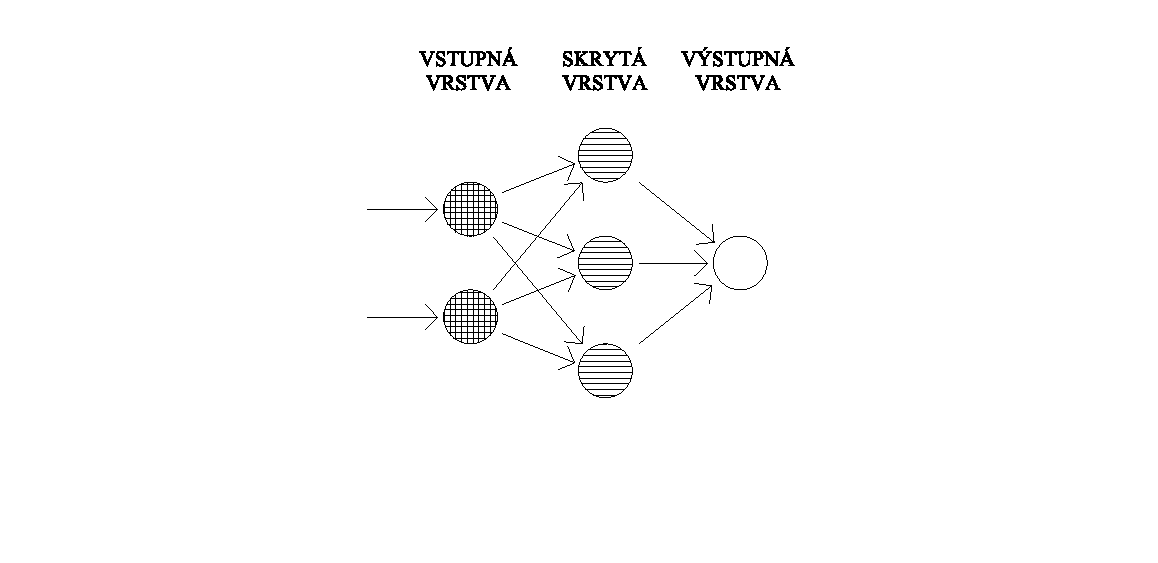
\includegraphics[width=1.0\textwidth]{images/siet.eps}
	\caption{Viacvrstvový perceptrón}
	\label{obrazok:neuronova-siet}
\end{figure}

V práci použijeme algoritmus učenia s učiteľom pomocou spätného šírenia chyby, čo je najpoužívanejší algoritmus učenia tohto druhu sietí. Viacvrstvový perceptrón realizuje nelineárnu funkciu z množiny možných vstupov do množiny príslušných výstupov. Už sme si predstavili algoritmus založený na lineárnom autoregresívnom modeli. Viacvrstvový perceptrón je rozšírením myšlienky lineárneho perceptrónu, ktorého možnosti sú teoreticky rovnaké ako možnosti autoregresívneho modelu. Motiváciou implementácie tohto algoritmu je otázka nakoľko si pri riešení nášho problému polepšíme prechodom z lineárneho na nelineárny model. Spoľahlivým zdrojom ďalších informácií o neurónových sietiach je \cite{Sima}. 

Podobne ako algoritmus založený na autoregresívnom modeli, bude aj tento pracovať po blokoch digitálnych vzoriek zo vstupného signálu o veľkosti $B$. Dôvodom pre blokové spracovávanie signálu naďalej zostáva menšia časová a pamäťová zložitosť výpočtu a jednotnejší hlasitostný aj frekvenčný charakter. Pre rámec algoritmu prepokladajme, že máme k dipozícii viacvrstvový perceptrón s počtom vstupných neurónov $N$, jedným výstupným neurónom a $H$ neurónmi v skrytej vrstve. Tréningy budú prebiehať v $T$-cyklovej iterácii s učiacim koeficientom $L$.

\subsection{Excitácia}
Majme daný vstupný poškodený signál $x$, prvý index $i$ a posledný index $j$ pre daný blok. Metóda si v prvom rade zostaví tréningovú množinu pre sieť zo vzoriek bloku. Táto tréningová množina pozostáva z dvojíc vstupného vektoru dĺžky $N$ a výstupného vektoru dĺžky $1$. Pre každú vzorku daného bloku zaradíme do tréningovej množiny dvojicu vstupného vektoru obsahujúceho $N$ bezprostredne predchádzajúcich vzoriek danej vzorke (v zachovanom poradí) a výstupného vektoru obsahujúceho len danú vzorku. Inými slovami, pre všetky indexy $k$ daného bloku zaradíme do tréningovej množiny dvojicu vstupného vektoru $\mathbf{a}_k$ a výstupného vektoru $\mathbf{b}_k$:
$$\mathbf{a}_k=\begin{bmatrix} 
x_{k-N} & x_{k-N+1} & \cdots & x_{k-1}\\
\end{bmatrix}^T,$$
$$\mathbf{b}_k=\begin{bmatrix} 
x_k\\ 
\end{bmatrix}^T.$$
Takto zostavenou tréningovou množinou natrénujeme našu sieť algoritmom učenia s učiteľom pomocou spätného šírenia chyby. 

Za pomoci natrénovanej získame vektor excitačného signálu pre daný blok:
$$\mathbf{e}=\begin{bmatrix} 
  e_i & e_{i+1} & \cdots & e_{j}\\
\end{bmatrix}^T$$ 
tak, že jednotlivé excitácie $e_k$ vyjadríme odčítaním predikovanej vzorky od poškodenej:
$$e_k = x_k - p_k.$$ 
V uvedenom vzťahu je predikovaná vzorka $p_k$ rovná jedinému prvku výstupného vektoru natrénovanej siete pre vstupný vektor $\mathbf{a}_k$.

\subsection{Korekcia}
Pri oprave poškodeného signálu algoritmus najskôr vykoná doprednú korekciu vstupného signálu $x$ s detekčným signálom $d$, po ktorej obdrží signál $f$. Ďalej vykoná druhú doprednú korekciu nad obrátenými signálmi $x$ a $d$, z ktorej opravený signál opätovne obráti vo výsledný opravený signál $r$. Proces získania signálu $r$ nazveme spätnou korekciou. Dopredná aj spätná korekcia prebieha postupne po blokoch poškodeného signálu o veľkosti $B$. Po tom, čo algoritmus získa dopredný aj spätný opravený signál vyhotoví finálnu korekciu v podobe signálu $y$. Princíp výpočtu finálnej korekcie z doprednej a spätnej si vysvetlíme na záver. Opíšme si najskôr metódu doprednej korekcie pre daný blok.

Majme vstupný poškodený signál $x$, jemu odpovedajúci detekčný signál $d$, prvý index $i$ a posledný index $j$ pre daný blok, na ktorom má prebehnúť dopredná korekcia. Ďalej majme signál $y$ obsahujúci dopredne opravené vzorky predchádzajúce danému bloku, získané z predošlých výpočtov. Metóda zostaví tréningovú množinu, do ktorej zaradí pre každú vzorku daného bloku, ktorá je spolu s jej $N$ bezprostredne predchadzajúcimi vzorkami v detekcii $d$ označená za nepoškodenú, dvojicu vstupného vektoru obsahujúceho $N$ bezprostredne predchádzajúcich vzoriek danej vzorke (v zachovanom poradí) a výstupného vektoru obsahujúceho len danú vzorku. Inými slovami, pre všetky indexy $k$ daného bloku, pre ktoré $k$-ta vzorka vstupného signálu spolu s jej $N$ bezprostredne predchádzajúcimi vzorkami sú v detekčnom signáli $d$ označené za nepoškodené, zahrnieme do tréningovej množiny dvojicu vstupného vektoru $\mathbf{a}_k$ a výstupného vektoru $\mathbf{b}_k$:
$$\mathbf{a}_k=\begin{bmatrix} 
x_{k-N} & x_{k-N+1} & \cdots & x_{k-1}\\ 
\end{bmatrix}^T,$$
$$\mathbf{b}_k=\begin{bmatrix} 
x_k\\ 
\end{bmatrix}^T.$$
Pripravenou tréningovou množinou natrénujeme našu sieť metódou učenia s učiteľom pomocou spätného šírenia chyby. 

V ďalšej časti algoritmu natrénovaná sieť poskytuje predikcie pre jednotlivé poškodené vzorky. Pri implementácii sa osvedčil dopredný prechod v rámci bloku s nahradením každej poškodenej vzorky predikovanou. Pri výpočte predikcie metóda počíta s predom vykonanými predikciami namiesto toho aby brala do úvahy poškodené vzorky. Výsledný dopredne opravený vektor získame vyjadrením:
$$\mathbf{f}=\begin{bmatrix} 
  f_i & f_{i+1} & \cdots & f_{j}\\
\end{bmatrix}^T$$ 
kde jednotlivé $f_k$ získame rekurzívne zo vzťahu:
$$f_k = \left\{\begin{array}{l l}
	y_k & \quad \text{$k<i$}\\
	x_k & \quad \text{$k\geq i$ a $d_k=0$}\\
	p_k & \quad \text{inak}\\
\end{array} \right.$$
kde predikcia $p_k$ je rovná jedinému prvku výstupného vektoru natrénovanej siete pre vstupný vektor:
$$\mathbf{f}_k=\begin{bmatrix} 
f_{k-N} & f_{k-N+1} & \cdots & f_{k-1}\\ 
\end{bmatrix}^T.$$

Konečný opravený signál $y$ získame zložením signálov doprednej $f$ a spätnej korekcie $r$ zo vzťahu:
$$y_n = \left\{\begin{array}{l l}
	x_n & \quad d_n = 0\\
	(1-\frac{o_n}{g_n+1}) \cdot f_n + (\frac{o_n}{g_n+1}) \cdot r_n & \quad d_n=1.\\
\end{array} \right.$$
Celočíselné pomocné signály $g$ a $o$ získame z detekčného signálu $d$ spôsobom popísaným v časti o naivnom algoritme.

\section{Detekčné brány}
V časti práci pojednávajúcej o obecnom algoritme pre reštaurovanie nahrávok poškodených lokálnymi znehodnoteniami bolo uvedené, že v druhej fáze detekcie sa na excitačný signál $e$ aplikuje detekčná brána. Úlohou detekčnej brány je určiť prvotnú detekciu poškodených vzoriek signálu $x$ v podobe binárneho detekčného signálu $\tilde{d}$. Popíšeme si princípy niekoľkých detekčných brán.

\subsection{Jednoduchá detekčná brána}
Jednoduchá detekčná brána v detekcii $\tilde{d}$ označí za poškodené tie vzorky, ktorých absolútna hodnota excitácie je väčšia než stanovený prah $T$. Detekciu získanú aplikáciou jednoduchej detekčnej brány na excitačný signál $e$ je možné formálne vyjadriť predpisom:
$$\tilde{d}_n = \left\{\begin{array}{l l}
	1 & \quad  |e_n|>T\\
	0 & \quad \text{inak}\\
\end{array} \right.$$
kde $T$ je prah brány. Veľkým nedostatkom jednoduchej detekčnej brány je absolútna neadaptívnosť voči charakteru excitačných signálov. Pre naše účely je jednoduchá detekčná brána takmer nepoužiteľná. V práci je predstavená len pre počiatočnú ilustráciu princípu fungovania brán.

\subsection{Detekčná brána smerodajnej odchýlky}
Nasledujúca brána je prispôsobivejšia než predchádzajúca jednoduchá. Detekčná brána smerodajnej odchýlky čiastočne prihliada pri detekcií poškodených vzoriek na charakter intenzity excitačného signálu. Detekčný signál $\tilde{d}$ získaný aplikáciou brány smerodajnej odchýlky na excitačný signál $e$ môžeme vyjadriť vzťahom:
$$\tilde{d}_n = \left\{\begin{array}{l l}
	1 & \quad |e_n|> P \cdot \sigma\\
	0 & \quad \text{inak.}\\
\end{array} \right.$$
kde $P$ je prahový parameter brány a $\sigma$ je smerodajná odchýlka excitačného signálu $e$. Jedným zo spôsobov ako získať smerodajú odchýlku $\sigma$ je priamym výpočtom zo známeho vzťahu:
$$\sigma=\sqrt{\frac{1}{N} \cdot \sum_{i=1}^N(e_i-\bar{e})^2}$$
kde $\bar{e}$ je priemerná hodnota vzorky excitačného signálu:
$$\bar{e}=\frac{1}{N} \cdot \sum_{i=1}^N(x_i).$$

Smerodajnú odchýlku $\sigma$ excitácií môžeme taktiež získať pomocou metódy robustnej aproximácie, ktorá bola zavedená Kleinerom a Martinom v ich práci \cite{Kleiner}. Kleiner-Martinova aproximačná metóda je v praxi bežne používana pre podobné účely. Jej predpis je nasledovný:
$$\sigma \approx \frac{med(|e|)}{0,6745}$$
kde $med(|e|)$ je medián absolútnych hodnôt vzoriek excitačného signálu $e$.
Detekčná brána smerodajnej odchýlky je vhodnou voľbou v situáciách, kedy nemá excitačný signál vo svojom priebehu premenlivú intenzitu.

\subsection{Adaptívna detekčná brána smerodajnej odchýlky}
Existuje mnoho spôsobov, akými by sme mohli získať bránu adaptívnu voči premenlivej intenzite excitácií. Jedno z možných riešení je nechať predošlú bránu počítať detekciu po blokoch vzoriek excitačného signálu. V takomto prípade by boli štandardné odchýlky a nimi určené prahy počítané lokálne zvlášť pre každý blok. Predstavme si vlastnú prispôsobivú bránu smerodajnej odchýlky, ktorá počíta detekciu vzhľadom na vzorkové okolie. Detekčný signál $\tilde{d}$ adaptívnej detekčnej brány smerodajnej odchýlky získame z excitačného signálu $e$ predpisom:
$$\tilde{d}_n = \left\{\begin{array}{l l}
	1 & \quad |e_n|> P \cdot \sigma_n\\
	0 & \quad \text{inak}\\
\end{array} \right.$$
kde $P$ je prahový parameter brány a $\sigma_n$ je lokálna smerodajná odchýlka excitácií:
$$\sigma_n=\sqrt{\frac{1}{2 \cdot R+1}\sum_{i=-R}^{R}(e_{n+C \cdot i} - \bar{e}_n})^2.$$
Vo vyššie uvedenom vzťahu je $R$ respektíve $C$ celočíselný koeficient vyjadrujúci rozsah respektíve decimáciu vzorkového okolia lokálneho výpočtu a $\bar{e}_n$ je lokálny priemer vzoriek excitácií:
$$\bar{e}_n=\frac{1}{2 \cdot R+1} \cdot \sum_{i=-R}^{R}e_{n+C \cdot i}.$$

Pre výpočet lokálnej smerodajnej odchýlky excitácií môžeme opäť použiť zmienenú aproximáčnú metódu navrhnutú Kleinerom a Martinom:
$$\sigma_n \approx \frac{med(|e_{n-C \cdot R}|, |e_{n-C \cdot (R-1)}|\cdots, |e_{n+C \cdot R}|)}{0,6745}.$$ 

Čo sa týka brán, nieje prispôsobivosť vždy žiadúcou vlastnosťou. Vhodnosť aplikácie adaptívnej brány záleží od pravidelnosti rozloženia lokálnych znehodnotení vo vstupnom poškodenom signáli.


\subsection{Systém dvoch prahov}
Systém detekčných brán, ktorého princíp si teraz opíšeme, je celkom univerzálny a je ho možné aplikovať na všetky v práci spomenuté brány. Jeho hlavnou myšlienkou je zaviesť dva prahy pre detekciu poškodených vzoriek z excitačného signálu. Prvý prah slúži k určeniu poškodenosti vzorky na začiatku postupnosti poškodených. Druhý prah slúži k určeniu poškodenosti vzorky uprostred postupnosti poškodených. 

Implementáciu systému do jednoduchej detekčnej brány získame zavedením dvoch prahov $T_1$, $T_2$ namiesto jediného $T$. Výsledný detekčný signál takto upravenej jednoduchej brány môžeme vyjadriť nasledovne:
$$\tilde{d}_n = \left\{\begin{array}{l l}
	1 & \quad \text{$|e_n|>T_1$ a $d_{n-1}=0$ alebo}\\
	 & \quad \text{$|e_n|>T_2$ a $d_{n-1}=1$}\\
	0 & \quad \text{inak}.\\
\end{array} \right.$$

Implementáciu systému do zvyšných z uvedených brán získame napríklad nahradením jediného prahového parametru $P$ dvomi novými $P_1$, $P_2$. 

Princíp dvoch prahov detekčných brán vznikol vďaka charakteru historických analógových médií a vlastnostiam im prislúchajúcich lokálnych znehodnotení. Tieto poškodenia mávajú zvyčajne začiatok intenzivnejší než svoj zvyšok, a to sa premieta aj do mnohých excitačných signálov.


\section{Detekčné modifikátory}
Poslednú nepovinnú fázu detekcie tvoria aplikácie detekčných modifikátorov. Tie pracujú s prvotnou detekciou poskytnutou detekčnou bránou v podobe signálu $\tilde{d}$. Cieľom aplikácií modifikátorov je skvalitnenie prvotných detekcií vo výsledný detekčný signál $d$. V rámci práce si predstavíme tri modifikátory, ktoré pri vhodnom použití redukujú nedostatky prvotných detekcií.

\subsection{Detekčný rozširovač}
Detekčný rozširovač upraví detekciu $\tilde{d}$ vo výslednú $d$ tak, že každú vzorku $\tilde{d}_n$ s danou binárnou hodnotou $L$ duplikuje na $P$ pozícií $dopredu$ alebo $dozadu$ prípadne $obecne$. Výslednú detekciu $d$ môžeme vyjadriť nasledovne:
$$d_n = \left\{\begin{array}{l l}
	L & \quad \text{$dopredu$ a $\exists i : (i \leq n$ a $\tilde{d}_i=L$ a $|n-i| \leq P$) alebo}\\
	& \quad \text{$dozadu$ a $\exists i : (i \geq n$ a $\tilde{d}_i=L$ a $|n-i| \leq P$) alebo}\\	
	& \quad \text{$obecne$ a $\exists i : (\tilde{d}_i=L$ a $|n-i| \leq P$)}\\
	1-L & \quad \text{inak}.\\
\end{array} \right.$$

\subsection{Detekčný prepájač}
Detekčný prepájač upraví detekciu $\tilde{d}$ tak, že každú dvojicu vzoriek $\tilde{d}_i$, $\tilde{d}_j$ s danou binárnou hodnotou $L$, ktorých vzájomná vzdialenosť je menšia ako parameter $P$, prepojí vo výslednom detekčnom signáli $d$ hodnotami $L$ na medzipozciách. Formálne môžeme výslednú detekciu $d$ vyjadriť:
$$d_n = \left\{\begin{array}{l l}
	L & \quad \min(\{\text{$j$ | $j \geq n$ a $\tilde{d}_j=L$} \}) - \max(\{\text{$i$ | $i \leq n$ a $\tilde{d}_i=L$} \}) \leq P\\
	1-L & \quad \text{inak}.\\
\end{array} \right.$$

\subsection{Detekčný posúvač}
Detekčný rozširovač upraví detekciu $\tilde{d}$ vo výslednú $d$ tak, že každú jeho vzorku posunie o $P$ pozícii $dopredu$ alebo $dozadu$. Výslednú detekciu $d$ môžeme vyjadriť nasledovne:
$$d_n = \left\{\begin{array}{l l}
	\tilde{d}_{n-P} & \quad dopredu\\
	\tilde{d}_{n+P} & \quad dozadu.\\
\end{array} \right.$$